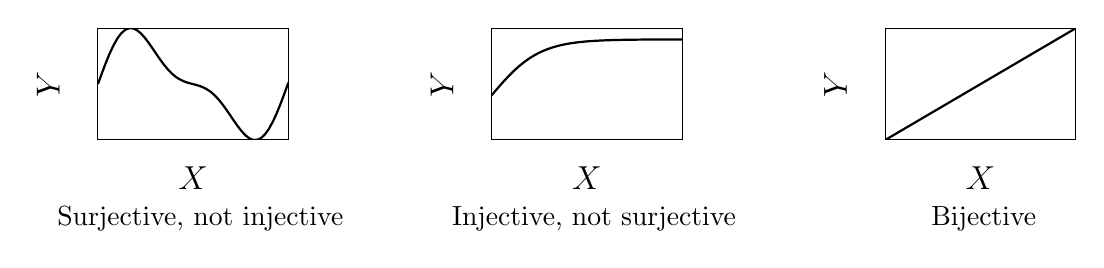
\begin{tikzpicture}

    % Surjective, not injective
    \begin{axis}[
            xshift=0cm,
            width=4cm, height=3cm,
            axis x line=box, axis y line=box,
            xtick=\empty, ytick=\empty,
            xlabel={$X$}, ylabel={$Y$},
            xlabel style={at={(0.5,-0.15)}, font=\large},
            ylabel style={at={(-0.15,0.5)}, font=\large},
            enlargelimits=false,
            % clip=true,
        ]
        \addplot[domain=0:6.3, samples=50, thick] {sin(deg(x))*0.6 + sin(deg(2*x))/4 + 1.1};
    \end{axis}
    \node at (1.3,-1.0) {Surjective, not injective};

    % Injective, not surjective
    \begin{axis}[
            xshift=5cm,
            width=4cm, height=3cm,
            axis x line=box, axis y line=box,
            xtick=\empty, ytick=\empty,
            xlabel={$X$}, ylabel={$Y$},
            xlabel style={at={(0.5,-0.15)}, font=\large},
            ylabel style={at={(-0.15,0.5)}, font=\large},
            enlargelimits=false,
            xmin=0, xmax=2,
            ymin=0, ymax=2,
        ]
        \addplot[domain=0:2, range=0:2, samples=50, thick] {tanh(2*x)+0.8};
    \end{axis}
    \node at (6.3,-1.0) {Injective, not surjective};

    % Bijective
    \begin{axis}[
            xshift=10cm,
            width=4cm, height=3cm,
            axis x line=box, axis y line=box,
            xtick=\empty, ytick=\empty,
            xlabel={$X$}, ylabel={$Y$},
            xlabel style={at={(0.5,-0.15)}, font=\large},
            ylabel style={at={(-0.15,0.5)}, font=\large},
            enlargelimits=false,
        ]
        \addplot[domain=0:2, samples=100, thick] {x+0.3};
    \end{axis}
    \node at (11.25,-1.0) {Bijective};

\end{tikzpicture}
